\documentclass[12pt]{article}

\usepackage[utf8x]{inputenc} % Включаем поддержку UTF8  
\usepackage[russian]{babel}  % Включаем пакет для поддержки русского языка  
\usepackage{hyperref}        % Для гиперссылок

% Математика
\usepackage{amsmath,amsfonts,amssymb,amsthm,mathtools} % AMS
\usepackage{icomma}
\usepackage{mathrsfs}

% Прога
\usepackage{etoolbox}
\usepackage{listings}

% Цвета
\usepackage{xcolor}

% Картинки
\usepackage{graphicx}
\graphicspath{ {./images/} }

\usepackage{tikzsymbols}

% Работа с таблицами
\usepackage{array,tabularx,tabulary,booktabs} % Дополнительная работа с таблицами
\usepackage{longtable}  % Длинные таблицы
\usepackage{multirow} % Слияние строк в таблице

% Нумерованные списки
\usepackage[shortlabels]{enumitem} % Разные лейблы

% Текст
\usepackage[normalem]{ulem}  % для зачеркивания текста

\newtheorem{property}{Свойство}
\newtheorem{consequence}{Следствие}[property]

\begin{document}
	
	\thispagestyle{empty}
	\begin{center}
		\textbf{ПРАВИТЕЛЬСТВО РОССИЙСКОЙ ФЕДЕРАЦИИ}
		
		\vspace{5ex}
		
		\textbf{Федеральное государственное автономное образовательное учреждение \\ высшего образования \\ <<Национальный исследовательский университет \\ <<Высшая школа экономики>>}
	\end{center}
	\vspace{5ex}
	
	\begin{center}
		Московский институт электроники и математики им. А.Н. Тихонова  
		
		\vspace{5ex}
		
		Департамент прикладной математики
		
		\vspace{10ex}
		\textbf{Отчёт \\ по лабораторной работе A1 \\ по курсу <<Компьютерный практикум>> \\ Задание № 13}
		\vspace{7ex}
		
	\end{center}
	
	\begin{center} 
		\begin{tabular}{| p{0.3\linewidth}| p{0.3\linewidth}| p{0.3\linewidth}|}
			\hline	
			ФИО студента & Номер группы & Дата \\  \hline
			& & \\  
			Кейер Александр \newline Петрович & БПМ-231 & 05.10.2023\\  
			& & \\  \hline		
		\end{tabular}
	\end{center}
	
	\begin{center}
		\vspace{3ex}
		
		\vfill
		
		\normalsize
		
		\textbf{Москва, 2023}
	\end{center}
	
	\newpage
	
	%---------------------------------------------------------------------------------
	
	\section*{Задание}
	
	
	\begin{enumerate}[a)]
		\item Вручную преобразовать десятичное в шестнадцатеричную и двоичную системы счисления. Число: $4015_{10}$
		
		\begin{table}[h]
			\centering
			\begin{tabularx}{0.88\textwidth}{| X| X| X|}
				\hline	
				Десятичная & Двоичная & 16-ричная \\  \hline
				$4015_{10}$ & $1111\:1010\:1111_2$  & $FAF_{16}$ \\   \hline	
				
			\end{tabularx}
		\end{table}
		
		\item В байте записано число. Необходимо перевести это число в двоичную и десятичную системы счисления в знаковом и беззнаковом представлении. Необходимо определить, какому символу кодовой таблицы соответствует данное число. Результаты занести в таблицу. Числа: D7h и 54h
	\end{enumerate}
	
	\newpage
	
	%---------------------------------------------------------------------------------
	
	\section*{Решение}\addcontentsline{toc}{section}{Введение}
	\subsection*{a)}
	
	\textbf{Переведем число $4015_{10}$ в двоичную систему счисления следующим образом:}
	\begin{enumerate}
		\item Будем делить $4015_{10}$ на 2 уголком: 
		
		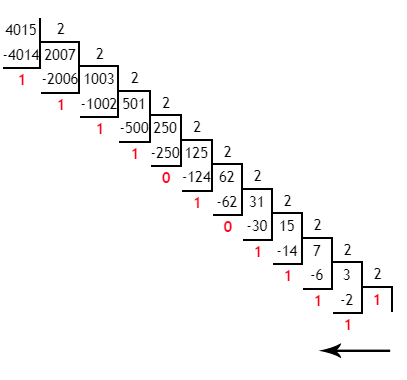
\includegraphics[width=1\linewidth]{angle}
		
		Таким образом, если записать полученные остатки и последнее частное, равное 1, справа налево, то получим: $$4015_{10 \to 2} = 1111\:1010\:1111_2$$
		\item Также проверим, как представляется число $4015_{10}$ в виде суммы степеней двоек:
		
		$$4015_{10} = 2^{11} + 2^{10} + 2^9 + 2^8 + 2^7 + 2^5 + 2^3 + 2^2 + 2^1 + 2^0 = 1111\:1010\:1111_2$$
		
	\end{enumerate}
	
	\textbf{Переведем число $4015_{10}$ в шестнадцатеричную систему счисления следующим образом:}
	\begin{enumerate}
		\item Будем делить $4015_{10}$ на 16 уголком: 
		
		\begin{center}
			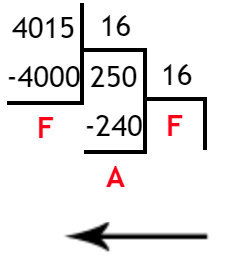
\includegraphics[width=125px]{angle16}
		\end{center}
		
		Таким образом, если записать полученные остатки и последнее частное, равное $F_{16}$, справа налево, то получим: $$4015_{10 \to 16} = FAF_{16}$$
		
		\item Сделаем проверку посредством разбиения двоичной записи числа $4015_{10}$ на четверки:
		$$
		\begin{array}{cccc}
			1111_2 & 1010_2 & 1111_2\\
			\downarrow & \downarrow & \downarrow \\
			F_{16} & A_{16} & F_{16}
		\end{array}
		$$
		
		$4015_{10} = 1111\:1010\:1111_2 = FAF_{16}$
	\end{enumerate}
	
	\newpage
	
	%---------------------------------------------------------------------------------
	
	\subsection*{b)}
	\begin{enumerate}
		\item Преобразуем числа из шестнадцатеричной системы счисления в двоичную посредством представления каждого знака числа, записанного в шестнадцатеричной системе счисления, четверкой цифр, образующих двоичную запись этого знака (символ h показывает, что данное число записано в шестнадцатеричной системе счисления):
		
		\begin{enumerate}
			\item $D7h = 1101\:0111_2$ 
			\item $54h = 0101\:0100_2$
		\end{enumerate}
		
		\item Для перевода числа в десятичную систему счисления в знаковом представлении необходимо понять, положительное это число или отрицательное. Посмотрим на знаковый бит: если он равен 1, то число отрицательное, если равен 0, то положительное.
		
		\begin{enumerate}
			\item \textbf{1}$101\:0111_2$ -- отрицательное число
			\item \textbf{0}$101\:0100_2$ -- положительное число
		\end{enumerate}
		
		Беззнаковое представление:
		
		\begin{enumerate}
			\item $1101\:0111_2 = 2^7 + 2^6 + 2^4 + 2^2 + 2^1 + 2^0 = 215_{10}$ 
			\item $0101\:0100_2 = 2^6 + 2^4 + 2^2 = 84_{10}$ 
		\end{enumerate}
		
		Знаковое представление чисел. Если число положительное, то его знаковое представление совпадает с беззнаковым, иначе необходимо взять старший бит со знаком минус:
		
		\begin{enumerate}
			\item $1101\:0111_2 = -2^7 + 2^6 + 2^4 + 2^2 + 2^1 + 2^0 = -41_{10}$ 
			\item $0101\:0100_2 = 2^6 + 2^4 + 2^2 = 84_{10}$ 
		\end{enumerate}
		
		\item С помощиью таблици ASCII найдем символы, которые соответствуют числам в дано:
	\end{enumerate} 
	
	\begin{center}
		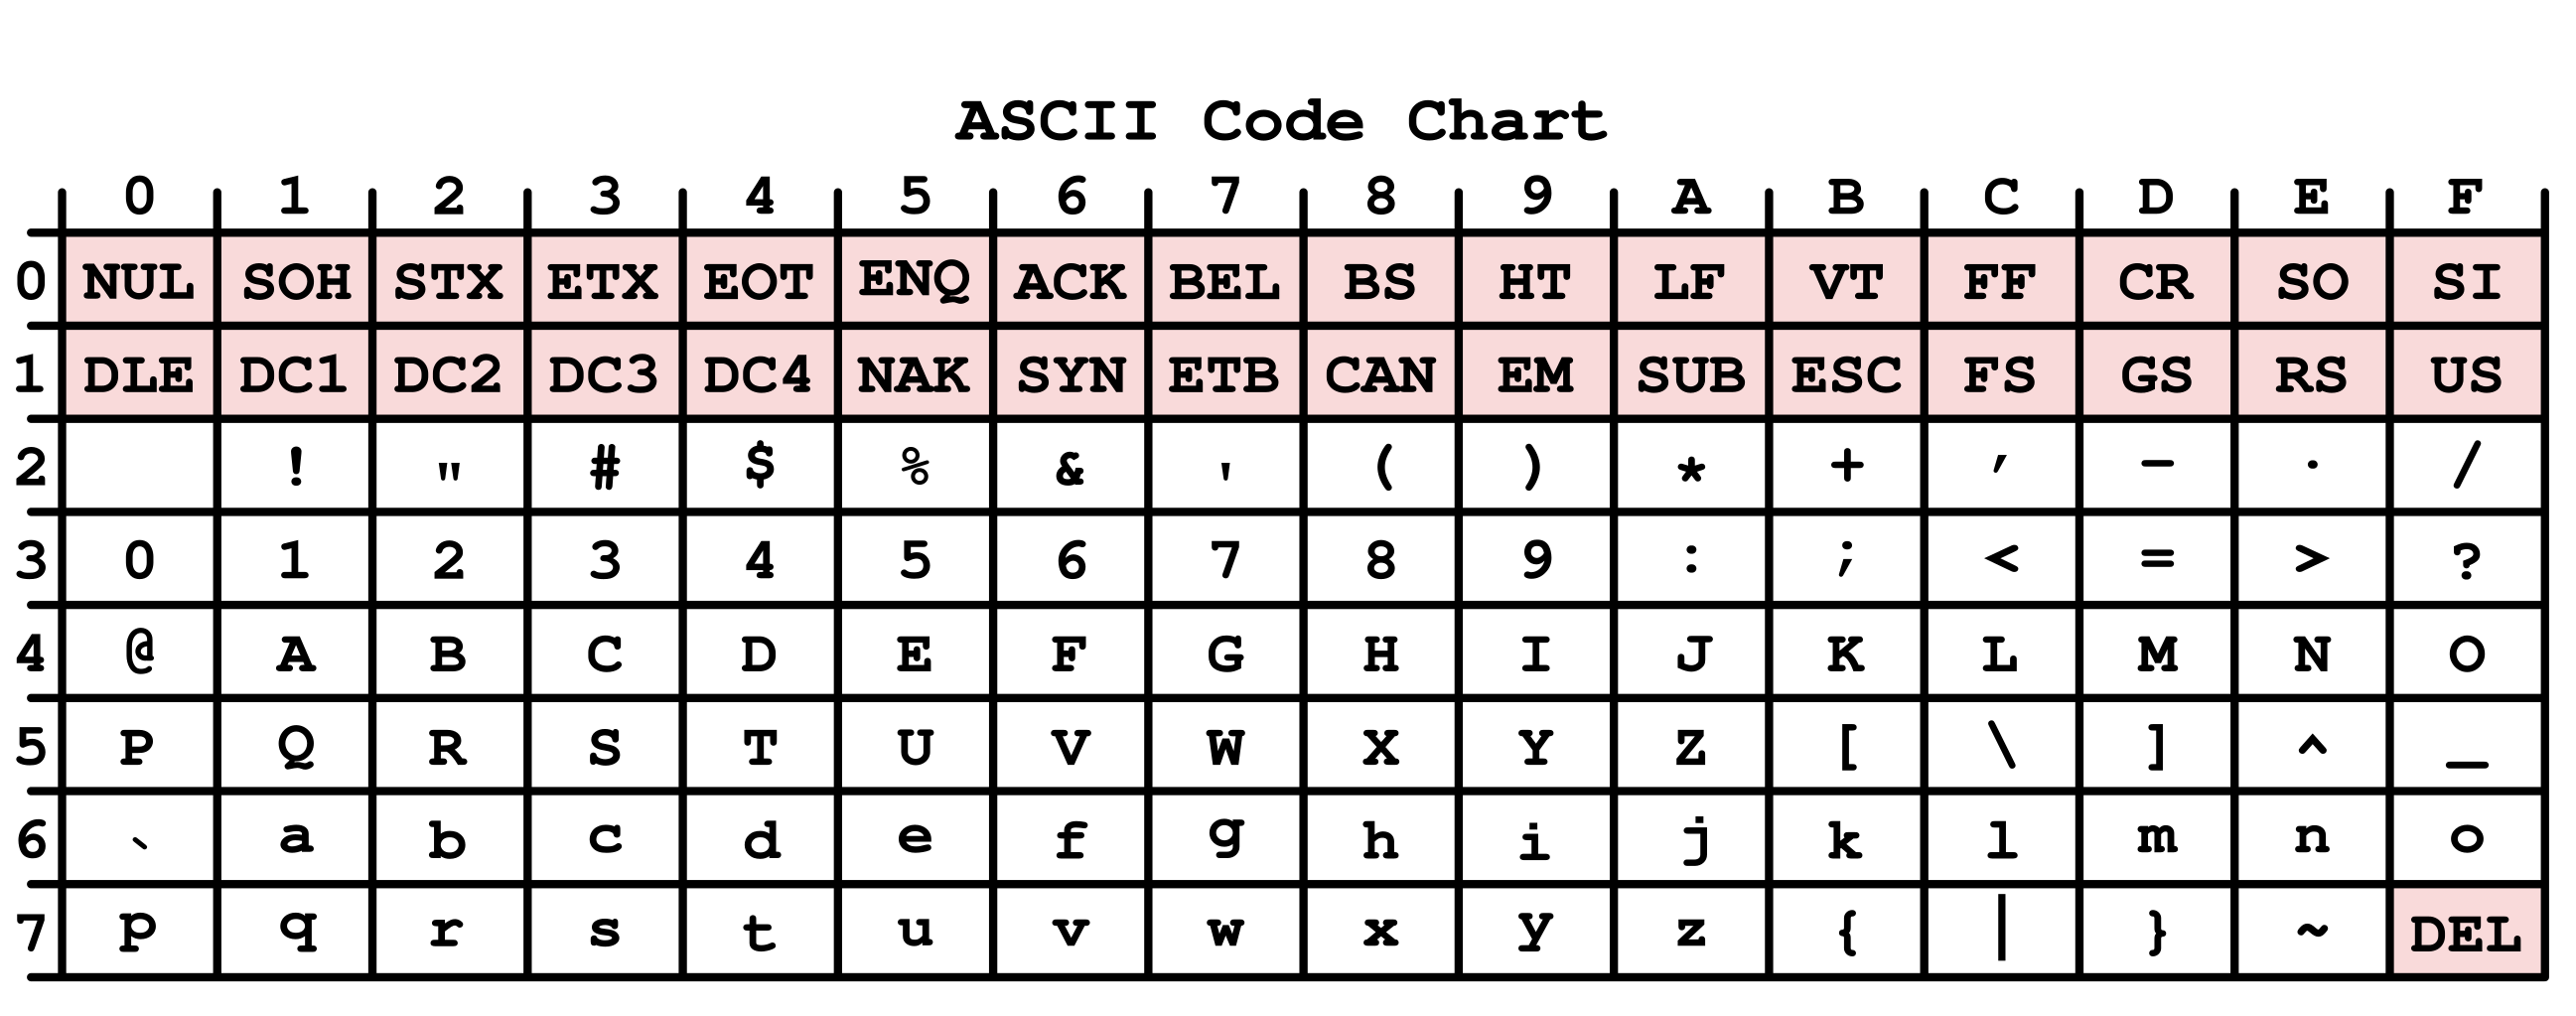
\includegraphics[width=355px]{ascii0}
		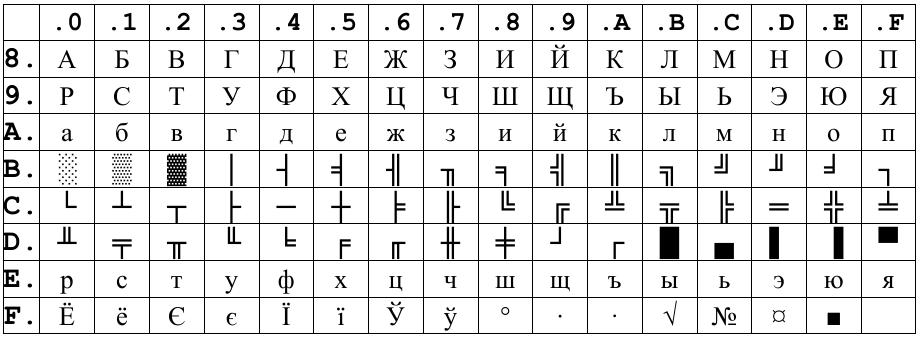
\includegraphics[width=350px]{ascii}
	\end{center}
	
	Числа соответствуют символам: \newline
	$$
	\begin{tabularx}{70px}{| X| X|}
		\hline	
		$D7h$ & \sout{||} \\ \hline
		$54h$ & $T$ \\ \hline	
	\end{tabularx}
	$$
\end{document}
